\documentclass[border=0mm]{standalone}

\usepackage{import}
\subimport{../../../}{preamble.tex}

\usepackage{tikz}
\usetikzlibrary{calc}
\usepackage{pgfplots}

\begin{document}

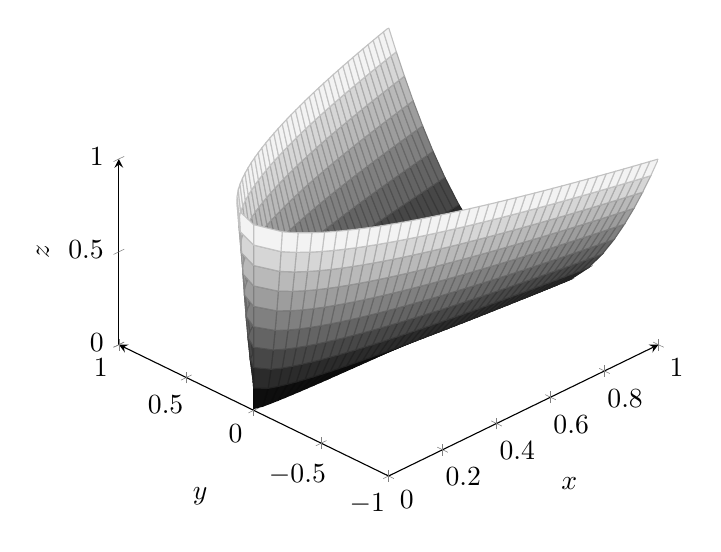
\begin{tikzpicture}
  \begin{axis}[
    view={-45}{45},
    axis lines=left,
    %axis on top,
    %grid=major,
    xlabel={$x$}, ylabel={$y$}, zlabel={$z$},
    xmin=0, xmax=1,
    %ymin=-1, ymax=1,
    zmin=0, zmax=1,
    samples=40,
    samples y=10,
    colormap/blackwhite,
    clip=true
    ]
    
    \addplot3 [surf, domain=1:0, y domain=0.01:1, opaque=1] ({x},{sqrt(x*y))},{y});
    \addplot3 [surf, domain=0:1, y domain=0.01:1] ({x},-{sqrt(abs(x*y))},{y});
    
  \end{axis}
\end{tikzpicture}

\end{document}

%%% Local Variables:
%%% mode: latex
%%% TeX-master: t
%%% End:
